\chapter{System Architecture and Technical Design}
\label{ch:architecture}

This chapter presents the system architecture and technical design decisions of the CHOYXONA.UZ application.
It covers the overall architectural approach, database structure and data modeling in Cloud Firestore, user interface design principles with responsive layout strategy, real-time data synchronization mechanisms, and Google Maps integration for geolocation services.


% =====================================================================
\section{General System Architecture}
\label{sec:system-arch}

The architecture of CHOYXONA.UZ follows a client-server model with Firebase services providing the complete backend infrastructure.
This architectural approach eliminates the need for deploying and maintaining custom server software, allowing development resources to focus on the user-facing application while leveraging Google's infrastructure for reliability, scalability, and global availability~\cite{moroney2017}.

The system architecture consists of three primary layers working together to deliver the application functionality:

\begin{enumerate}
  \item \textbf{Presentation layer} --- implemented entirely in Flutter, this layer handles all user interface rendering, user interaction, and navigation logic that creates the visual experience users interact with.
  \item \textbf{Business logic layer} --- combines client-side Dart code executing within the Flutter application with Firebase Cloud Functions executing on Google's servers for operations requiring elevated privileges or triggered by database events.
  \item \textbf{Data layer} --- managed by Cloud Firestore for structured data and Cloud Storage for binary files (images, documents), this layer persists all application state and user-generated content.
\end{enumerate}

Client applications communicate with Firebase services through official SDKs that handle authentication, network connectivity, data serialization, and local caching.
The Firebase SDK manages network connections automatically, retrying failed requests with exponential backoff and queuing write operations when offline for later synchronization~\cite{firebase_firestore2024}.
This automatic handling of network unreliability significantly reduces application code complexity while improving user experience in conditions with intermittent connectivity --- a particularly relevant consideration in Uzbekistan where mobile network quality varies by region.

The Flutter application organizes code following a \textbf{feature-based structure} that groups related files by functionality rather than by technical type.
The main source directories include:

\begin{itemize}
  \item \texttt{models/} --- Dart classes representing business entities (users, establishments, bookings);
  \item \texttt{services/} --- classes encapsulating Firebase interactions and backend communication;
  \item \texttt{screens/} --- UI components organized by feature area (authentication, home, search, booking, profile);
  \item \texttt{widgets/} --- reusable UI components used across multiple screens;
  \item \texttt{core/} --- shared utilities including theme definitions, constants, and helper functions.
\end{itemize}

This organization follows the separation of concerns principle recommended by Martin~\cite{martin2017}, enabling clear code boundaries while keeping related files together for easier navigation and maintenance.

The high-level interaction between system components is illustrated in \cref{fig:system-arch}.

\begin{figure}[htbp]
  \centering
  \begin{tikzpicture}[
    box/.style={draw, rounded corners=4pt, minimum width=3.2cm, minimum height=1cm, align=center, font=\small},
    layer/.style={draw, dashed, rounded corners=6pt, inner sep=8pt, fill=#1!5},
    arr/.style={->, thick, >=Stealth},
    node distance=1cm and 1.5cm
  ]
    % Presentation Layer
    \node[layer=blue, minimum width=12cm, minimum height=2.8cm, label={[font=\small\bfseries]above:Presentation Layer (Flutter)}] (pl) {};
    \node[box, fill=blue!15] at (-3.5,0) (screens) {Screens\\(UI Pages)};
    \node[box, fill=blue!15] at (0,0) (widgets) {Widgets\\(Reusable UI)};
    \node[box, fill=blue!15] at (3.5,0) (providers) {Providers\\(State Mgmt)};
    \draw[arr] (screens) -- (widgets);
    \draw[arr] (screens) -- (providers);

    % Business Logic Layer  
    \node[layer=green, minimum width=12cm, minimum height=1.4cm, label={[font=\small\bfseries]above:Business Logic Layer}] (bl) at (0,-3.2) {};
    \node[box, fill=green!15] at (-2.5,-3.2) (services) {Services\\(Dart)};
    \node[box, fill=green!15] at (2.5,-3.2) (functions) {Cloud\\Functions};

    % Data Layer
    \node[layer=orange, minimum width=12cm, minimum height=1.4cm, label={[font=\small\bfseries]above:Data Layer (Firebase)}] (dl) at (0,-5.8) {};
    \node[box, fill=orange!15] at (-3.5,-5.8) (firestore) {Cloud\\Firestore};
    \node[box, fill=orange!15] at (0,-5.8) (storage) {Cloud\\Storage};
    \node[box, fill=orange!15] at (3.5,-5.8) (auth) {Firebase\\Auth};

    % Arrows
    \draw[arr] (providers) -- (services);
    \draw[arr] (services) -- (firestore);
    \draw[arr] (services) -- (storage);
    \draw[arr] (services) -- (auth);
    \draw[arr] (functions) -- (firestore);
  \end{tikzpicture}
  \caption{High-level system architecture of CHOYXONA.UZ showing three-layer organization.}
  \label{fig:system-arch}
\end{figure}

The three-layer architecture ensures that changes to one layer have minimal impact on others.
For example, switching from Cloud Firestore to a different database would require changes only in the services layer, leaving the presentation layer and its associated state management intact.
Similarly, UI redesign affects only the presentation layer without requiring modifications to business logic or data access code.


% =====================================================================
\section{Database Design and Data Model}
\label{sec:database}

The database design in Cloud Firestore utilizes several collections to store application data, with each collection containing documents that represent individual entities.
Firestore's NoSQL document model provides flexibility for varying data shapes without requiring schema migrations~\cite{firebase_firestore2024}.

\subsection{Primary Collections}
\label{subsec:collections}

The \textbf{users} collection contains a document for each registered user, identified by their Firebase Authentication UID.
User documents store:
\begin{itemize}
  \item Profile information: \texttt{displayName}, \texttt{email}, \texttt{phoneNumber}, \texttt{photoURL};
  \item Role assignment: possible values including \texttt{user}, \texttt{admin}, and \texttt{superadmin};
  \item Associated establishment identifier (for administrator accounts);
  \item User preferences: language selection and notification settings;
  \item Account status and creation timestamp.
\end{itemize}

The \textbf{choyxonas} collection holds establishment data with each document representing one restaurant or teahouse.
Establishment documents contain essential information including name, description, and establishment type categorized as traditional teahouse, national cuisine, European cuisine, or mixed menu.
Location data includes address text, region identifier for filtering, and geographic coordinates stored as a \texttt{GeoPoint} for map display and distance calculations.
Contact information encompasses phone numbers, social media links, and website URL.
Operating schedule stores hours for each day of the week.
Amenities list features such as Wi-Fi, parking, and private rooms using a string array.

The \textbf{bookings} collection tracks reservations with documents linking users to establishments at specific times.
Booking documents contain references to the user and establishment documents, enabling queries from either direction.
Temporal data includes the booking date, start time, and expected duration.
The status field tracks the booking lifecycle through states: \textit{pending} $\to$ \textit{confirmed} $\to$ \textit{completed} (or \textit{cancelled}/\textit{no-show}).
This lifecycle is visualized in \cref{fig:booking-lifecycle}.

\begin{figure}[htbp]
  \centering
  \begin{tikzpicture}[
    state/.style={draw, rounded corners=6pt, minimum width=2.2cm, minimum height=0.8cm, align=center, font=\small, fill=#1!15},
    arr/.style={->, thick, >=Stealth},
    node distance=2.5cm
  ]
    \node[state=yellow] (pending)   {Pending};
    \node[state=green,  right=of pending]   (confirmed) {Confirmed};
    \node[state=blue,   right=of confirmed] (completed) {Completed};
    \node[state=red,    below=1.2cm of confirmed] (cancelled) {Cancelled};
    \node[state=orange, right=of cancelled] (noshow)    {No-show};

    \draw[arr] (pending)   -- node[above,font=\scriptsize]{admin confirms} (confirmed);
    \draw[arr] (confirmed) -- node[above,font=\scriptsize]{visit done} (completed);
    \draw[arr] (pending)   |- node[near end,left,font=\scriptsize]{user/admin} (cancelled);
    \draw[arr] (confirmed) -- node[left,font=\scriptsize]{cancel} (cancelled);
    \draw[arr] (confirmed) -| node[near end,above,font=\scriptsize]{missed} (noshow);
  \end{tikzpicture}
  \caption{Booking status lifecycle showing state transitions from creation to completion.}
  \label{fig:booking-lifecycle}
\end{figure}

Additional collections support auxiliary features:
\begin{itemize}
  \item \textbf{reviews} --- user ratings and text feedback with references to user and establishment;
  \item \textbf{orders} --- in-venue ordering tracking menu items, quantities, and order status;
  \item \textbf{notifications} --- push notification history for each user;
  \item \textbf{promotions} --- marketing campaigns and special offers from establishments.
\end{itemize}


\subsection{Data Modeling Strategies}
\label{subsec:data-modeling}

Document structure was designed to optimize common query patterns while minimizing data redundancy and read costs.
\textbf{Denormalization} is employed strategically where read performance justifies data duplication.
For example, booking documents embed the establishment name rather than only storing a reference, avoiding an additional Firestore read when displaying booking history.
The tradeoff is that establishment name changes require updating associated bookings, handled through batch operations~\cite{firebase_firestore2024}.

\textbf{Subcollections} organize hierarchical data: menu items exist as a subcollection under each establishment document rather than as a top-level collection, ensuring menu queries are naturally scoped to a single establishment.
This also means that loading establishment list data does not inadvertently load all menu items as well.

The entity-relationship structure of the primary data model is shown in \cref{tab:er-model}.

\begin{table}[htbp]
\caption{Entity-relationship summary of the CHOYXONA.UZ data model}
\label{tab:er-model}
\centering
\small
\begin{tabular}{llll}
\toprule
\textbf{Entity (Collection)} & \textbf{Key Fields} & \textbf{Relationships} & \textbf{Subcollections} \\
\midrule
\texttt{users}      & name, email, role, phone & $\to$ choyxonas (admin) & favorites \\
\texttt{choyxonas}  & name, location, type, status & $\to$ users (admin ref) & menu, rooms \\
\texttt{bookings}   & date, time, status, guests & $\to$ users, choyxonas & --- \\
\texttt{reviews}    & rating, text, timestamp & $\to$ users, choyxonas & --- \\
\texttt{notifications} & title, body, read status & $\to$ users & --- \\
\bottomrule
\end{tabular}
\end{table}


\subsection{Indexing and Security}
\label{subsec:indexing-security}

\textbf{Indexing strategy} considers the filtering, sorting, and pagination operations required by the application.
Firestore automatically creates indexes for single-field queries, but composite indexes must be explicitly defined for multi-field queries.
The \texttt{firestore.indexes.json} configuration file defines composite indexes supporting common queries such as:
\begin{itemize}
  \item Filtering establishments by region while sorting by rating;
  \item Querying bookings for an establishment ordered by date;
  \item Filtering reviews by establishment while sorting by recency.
\end{itemize}

\textbf{Security rules} implement role-based access control at the database level.
Rules execute on Firebase servers, ensuring enforcement regardless of client behavior~\cite{firebase_firestore2024}.
The access control matrix is summarized in \cref{tab:security-rules}.

\begin{table}[htbp]
\caption{Firestore security rules --- access control matrix by user role}
\label{tab:security-rules}
\centering
\small
\begin{tabular}{lcccc}
\toprule
\textbf{Collection} & \textbf{Operation} & \textbf{User} & \textbf{Admin} & \textbf{Super Admin} \\
\midrule
users      & Read own    & \checkmark & \checkmark & \checkmark \\
users      & Write own   & \checkmark & \checkmark & \checkmark \\
users      & Read others & ---        & ---        & \checkmark \\
choyxonas  & Read        & \checkmark & \checkmark & \checkmark \\
choyxonas  & Write own   & ---        & \checkmark & \checkmark \\
bookings   & Create      & \checkmark & ---        & --- \\
bookings   & Read own    & \checkmark & \checkmark$^*$ & \checkmark \\
bookings   & Update status & ---      & \checkmark$^*$ & \checkmark \\
reviews    & Create      & \checkmark & ---        & --- \\
reviews    & Read        & \checkmark & \checkmark & \checkmark \\
\bottomrule
\multicolumn{5}{l}{\scriptsize $^*$ Admin access limited to their own establishment's data.}
\end{tabular}
\end{table}


% =====================================================================
\section{User Interface Design and Responsive Approach}
\label{sec:ui-design}

The user interface of CHOYXONA.UZ adheres to Material Design~3 guidelines while incorporating elements that resonate with the target cultural context~\cite{material2024}.
The design philosophy prioritizes clarity, accessibility, and efficient task completion across all user journeys.

\subsection{Visual Design System}
\label{subsec:visual-design}

The visual design employs a carefully selected color palette balancing tradition with modernity.
The primary color, a warm earthy brown tone, evokes the aesthetic of traditional teahouses while maintaining sufficient contrast for accessibility.
Both \textbf{light and dark themes} are fully supported, responding to user preference or system settings.

The \texttt{ThemeProvider} implementation uses Flutter's Provider pattern to manage theme state.
At startup, the provider checks stored preference; if none exists, it follows system setting.
Users can explicitly select light, dark, or automatic mode through the settings screen.
Theme changes take effect immediately without restart~\cite{flutter_state2024}.

Typography follows Material Design recommendations with \texttt{Roboto} as the primary typeface for its readability across sizes and weights.
Font scaling respects system accessibility settings, ensuring users who configure larger text see appropriately scaled text without layout breakage~\cite{nielsen2012}.

\subsection{Navigation Architecture}
\label{subsec:navigation}

Navigation implements a \textbf{bottom navigation bar} for five primary destinations:
\begin{enumerate}
  \item \texttt{Home} --- featured establishments and personalized content;
  \item \texttt{Map View} --- geographic discovery with interactive map;
  \item \texttt{Favorites} --- saved establishments for quick access;
  \item \texttt{Orders} --- booking history and management;
  \item \texttt{Profile} --- account and preference management.
\end{enumerate}

Secondary navigation uses stack-based routing through Navigator~2.0 for deeper navigation flows: from Home to establishment details to booking flow, and back.
Within screens, tabs organize related content --- the establishment detail screen uses tabs to separate Overview, Menu, and Reviews sections~\cite{wasserman2010}.

\subsection{Responsive Layout Strategy}
\label{subsec:responsive}

Responsive design ensures appropriate layouts across device sizes from compact phones to large tablets.
Key breakpoints distinguish layout modes as shown in \cref{tab:breakpoints}.

\begin{table}[htbp]
\caption{Responsive layout breakpoints and corresponding design adaptations}
\label{tab:breakpoints}
\centering
\small
\begin{tabular}{lcl}
\toprule
\textbf{Layout} & \textbf{Width (dp)} & \textbf{Adaptation} \\
\midrule
Compact (phone portrait)  & $< 600$     & Single-column, full-width cards \\
Medium (tablet portrait)  & $600$--$840$  & Two-column grid for lists \\
Expanded (tablet landscape) & $> 840$   & Master-detail side-by-side \\
\bottomrule
\end{tabular}
\end{table}

\texttt{MediaQuery} provides device dimensions enabling conditional layout adjustments, while \texttt{LayoutBuilder} provides parent constraints for components that need to adapt to their allocation~\cite{flutter_arch2024}.

\subsection{Localization}
\label{subsec:localization}

Localization extends beyond text translation to encompass all culture-specific aspects.
The \texttt{EasyLocalization} package manages translation files and runtime language switching.
The application supports three languages:
\begin{itemize}
  \item \textbf{Uzbek} --- primary local language;
  \item \textbf{Russian} --- widely understood due to historical context;
  \item \textbf{English} --- for international visitors and expatriates.
\end{itemize}

Date/time formats, currency displays, and number formatting all adjust to locale conventions.
Language preference persists locally using \texttt{SharedPreferences}, loading on subsequent launches.
The initial language defaults to the device's locale if supported, otherwise falling back to Russian~\cite{sommerville2015}.


% =====================================================================
\section{Real-time Synchronization and Data Streaming}
\label{sec:realtime}

Real-time data synchronization represents a cornerstone feature of CHOYXONA.UZ, differentiating it from simple request-response applications and enabling experiences that feel immediately responsive to changing information~\cite{firebase_firestore2024}.

Traditional applications interact with servers through request-response patterns: the client sends a request, the server returns a response, and the client displays the result.
To see updates, users must explicitly refresh.
This pattern creates poor experiences when timeliness matters --- a user viewing available booking times might make decisions based on stale information if another user has just taken a slot.

Firestore provides an alternative through \textbf{real-time listeners}.
Clients establish persistent subscriptions to documents or collections, receiving automatic updates whenever data changes on the server.
Flutter's reactive model integrates naturally through the \texttt{StreamBuilder} widget, which rebuilds its child whenever the stream emits a new value~\cite{flutter_arch2024}.

In CHOYXONA.UZ, real-time synchronization applies to several key scenarios:
\begin{itemize}
  \item \textbf{Availability display}: when customers view establishment slots, changes from other bookings appear immediately.
  \item \textbf{Admin dashboard}: today's bookings stream updates as new reservations arrive.
  \item \textbf{Reviews}: new reviews appear in real-time as submitted.
  \item \textbf{Notifications}: new notifications surface without manual refresh.
\end{itemize}

The \texttt{DataSyncProvider} class implements centralized stream management for data shared across multiple screens.
Rather than creating new subscriptions each time a widget needs data, the provider maintains canonical streams that multiple consumers share.
This reduces Firebase read operations since multiple listeners to a single stream count as one active listener, not multiple~\cite{khawas2018}.

\textbf{Offline persistence}, enabled by default in the Firestore SDK, extends usability when connectivity is unavailable.
The SDK maintains a local cache of recently accessed documents.
When offline, reads return cached data; writes queue locally and synchronize when connectivity resumes.

For booking operations requiring atomicity, \textbf{Firestore transactions} ensure consistent results.
A booking transaction reads current bookings for the requested time, verifies no conflict exists, and creates the new booking atomically.
If another booking was created between the read and write, the transaction retries with fresh data.
\textbf{Optimistic updates} improve perceived responsiveness --- the UI immediately displays a pending booking while the write proceeds asynchronously, reverting only if the write fails~\cite{firebase_firestore2024}.


% =====================================================================
\section{Google Maps Integration and Geolocation Services}
\label{sec:maps}

Geographic functionality significantly enhances discovery and navigation in CHOYXONA.UZ, enabling users to find establishments near their current location, visualize options on a map, and obtain directions~\cite{sommerville2015}.

Integration with Google Maps Platform provides the foundation.
The \texttt{google\_maps\_flutter} package renders interactive maps within the Flutter application as native components, providing smooth gesture-based panning and zooming.

\begin{figure}[htbp]
  \centering
  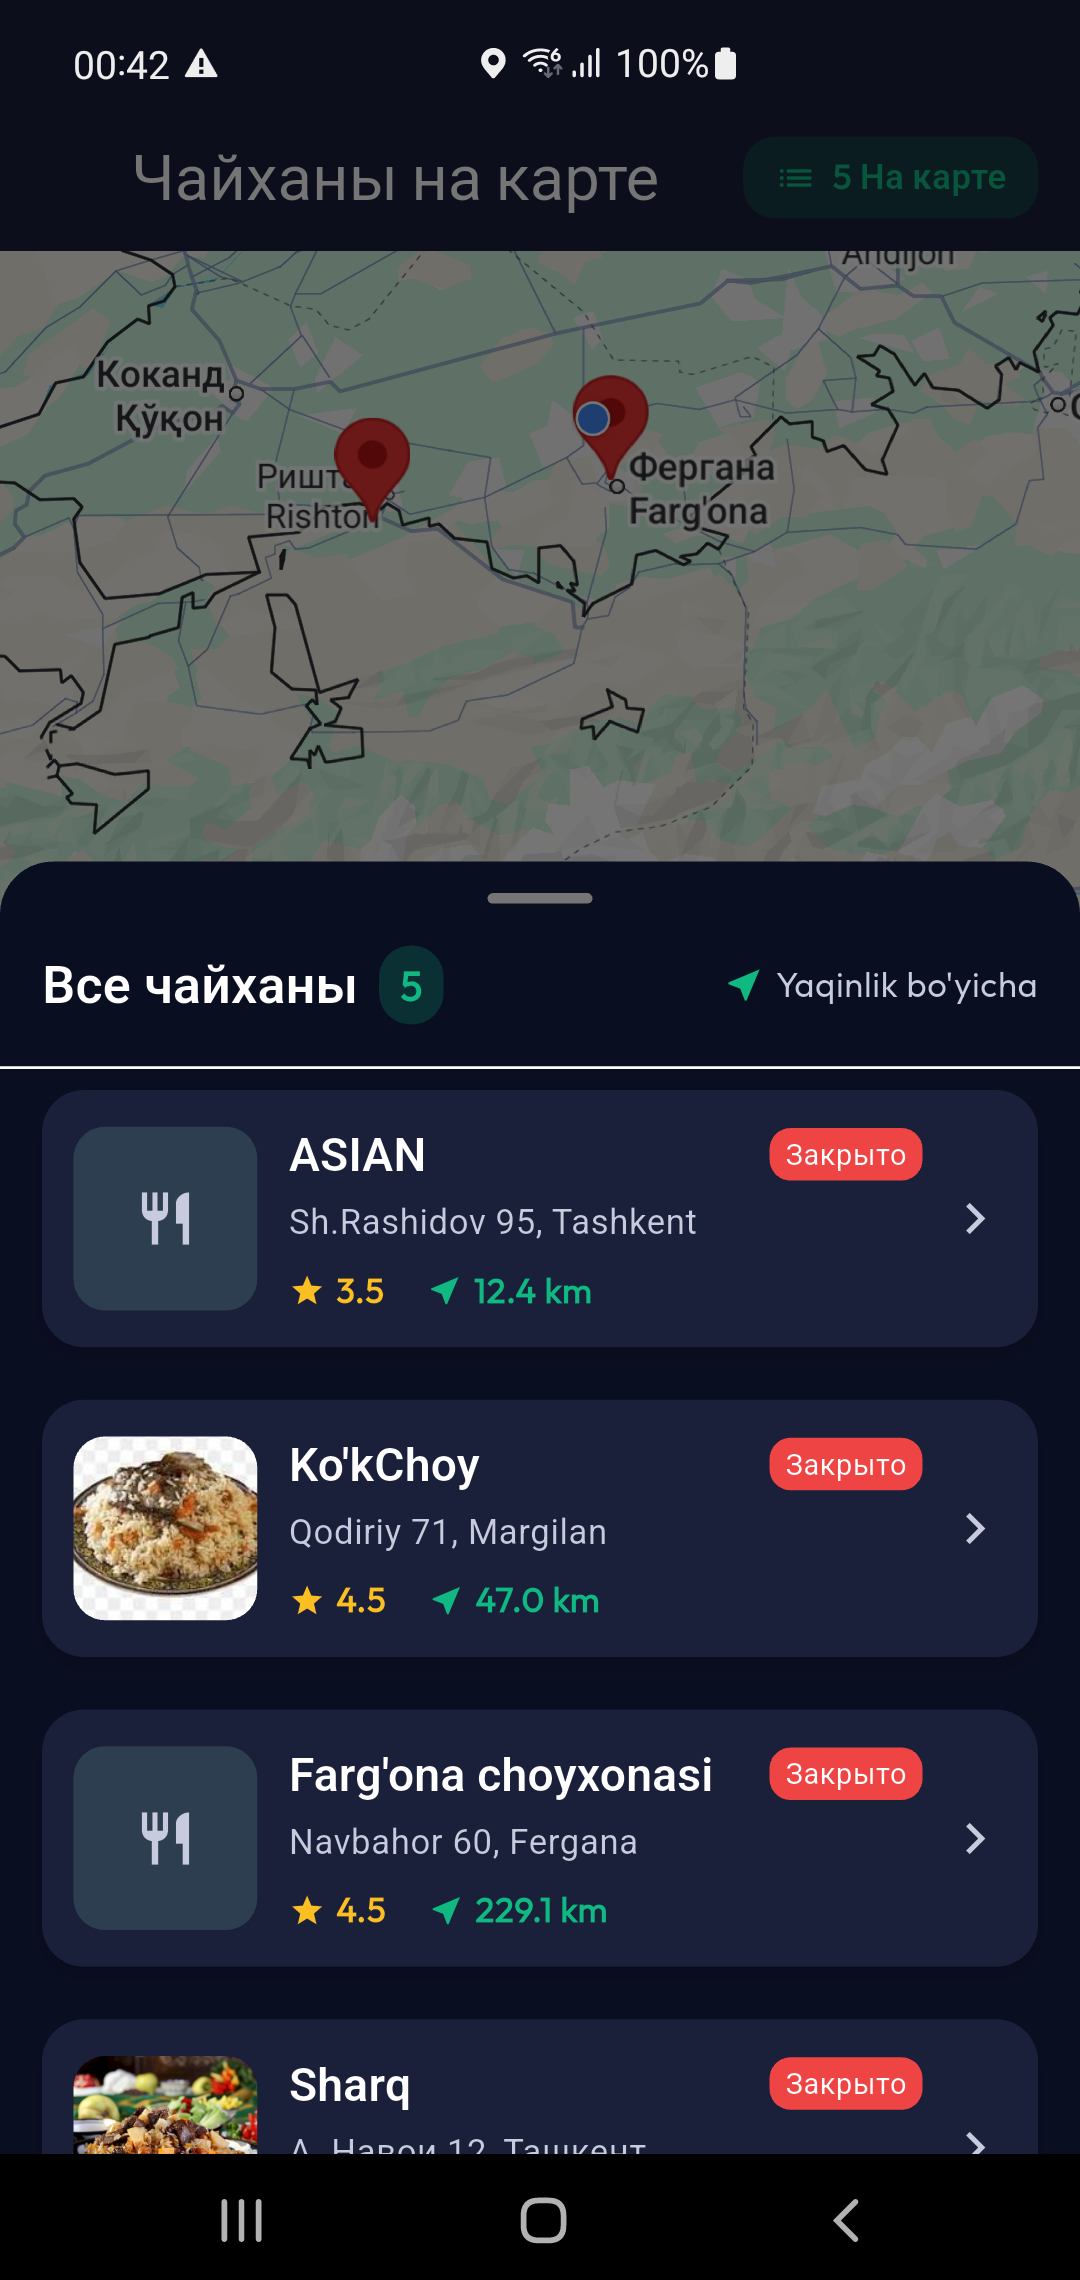
\includegraphics[width=0.4\textwidth]{b_chapters/chapter2/assets/google_maps.png}
  \figsource{CHOYXONA.UZ application screenshot.}
  \caption{Map interface showing establishment locations with markers across Uzbekistan.}
  \label{fig:google-maps}
\end{figure}

As shown in \cref{fig:google-maps}, establishment locations appear as markers positioned according to their geographic coordinates.
Custom marker images distinguish establishment types visually.
Tapping a marker displays an info window with essential information including name, rating, and price range, with navigation to the full detail screen.

Location services utilize the \texttt{geolocator} package to access the device's GPS.
Location access requires explicit user permission, handled through a permission request flow.
When granted, the user's current location becomes the default center for map views and basis for sorting by proximity.
Distance calculation employs the \textbf{Haversine formula} for great-circle distance between coordinates:

\begin{equation}
  d = 2r \cdot \arcsin\!\left(\sqrt{\sin^2\!\left(\frac{\varphi_2-\varphi_1}{2}\right) + \cos\varphi_1 \cdot \cos\varphi_2 \cdot \sin^2\!\left(\frac{\lambda_2-\lambda_1}{2}\right)}\right)
  \label{eq:haversine}
\end{equation}

\noindent where $r$ is Earth's radius, $\varphi$ is latitude, and $\lambda$ is longitude in radians.
This provides accurate measurements for the typical distances involved in local restaurant search.

\textbf{Region-based filtering} provides geographic organization without requiring location permission.
The application presents a region selector with major Uzbek cities: Tashkent, Samarkand, Bukhara, Namangan, Andijan, Fergana, and others.
This supports users planning visits to unfamiliar areas~\cite{jia2014}.

\textbf{Directions integration} constructs intent URIs that open external navigation applications (Google Maps on Android, Apple Maps on iOS), respecting user choice of navigation tools and providing full navigation functionality without duplicating turn-by-turn capabilities.

\begin{figure}[htbp]
  \centering
  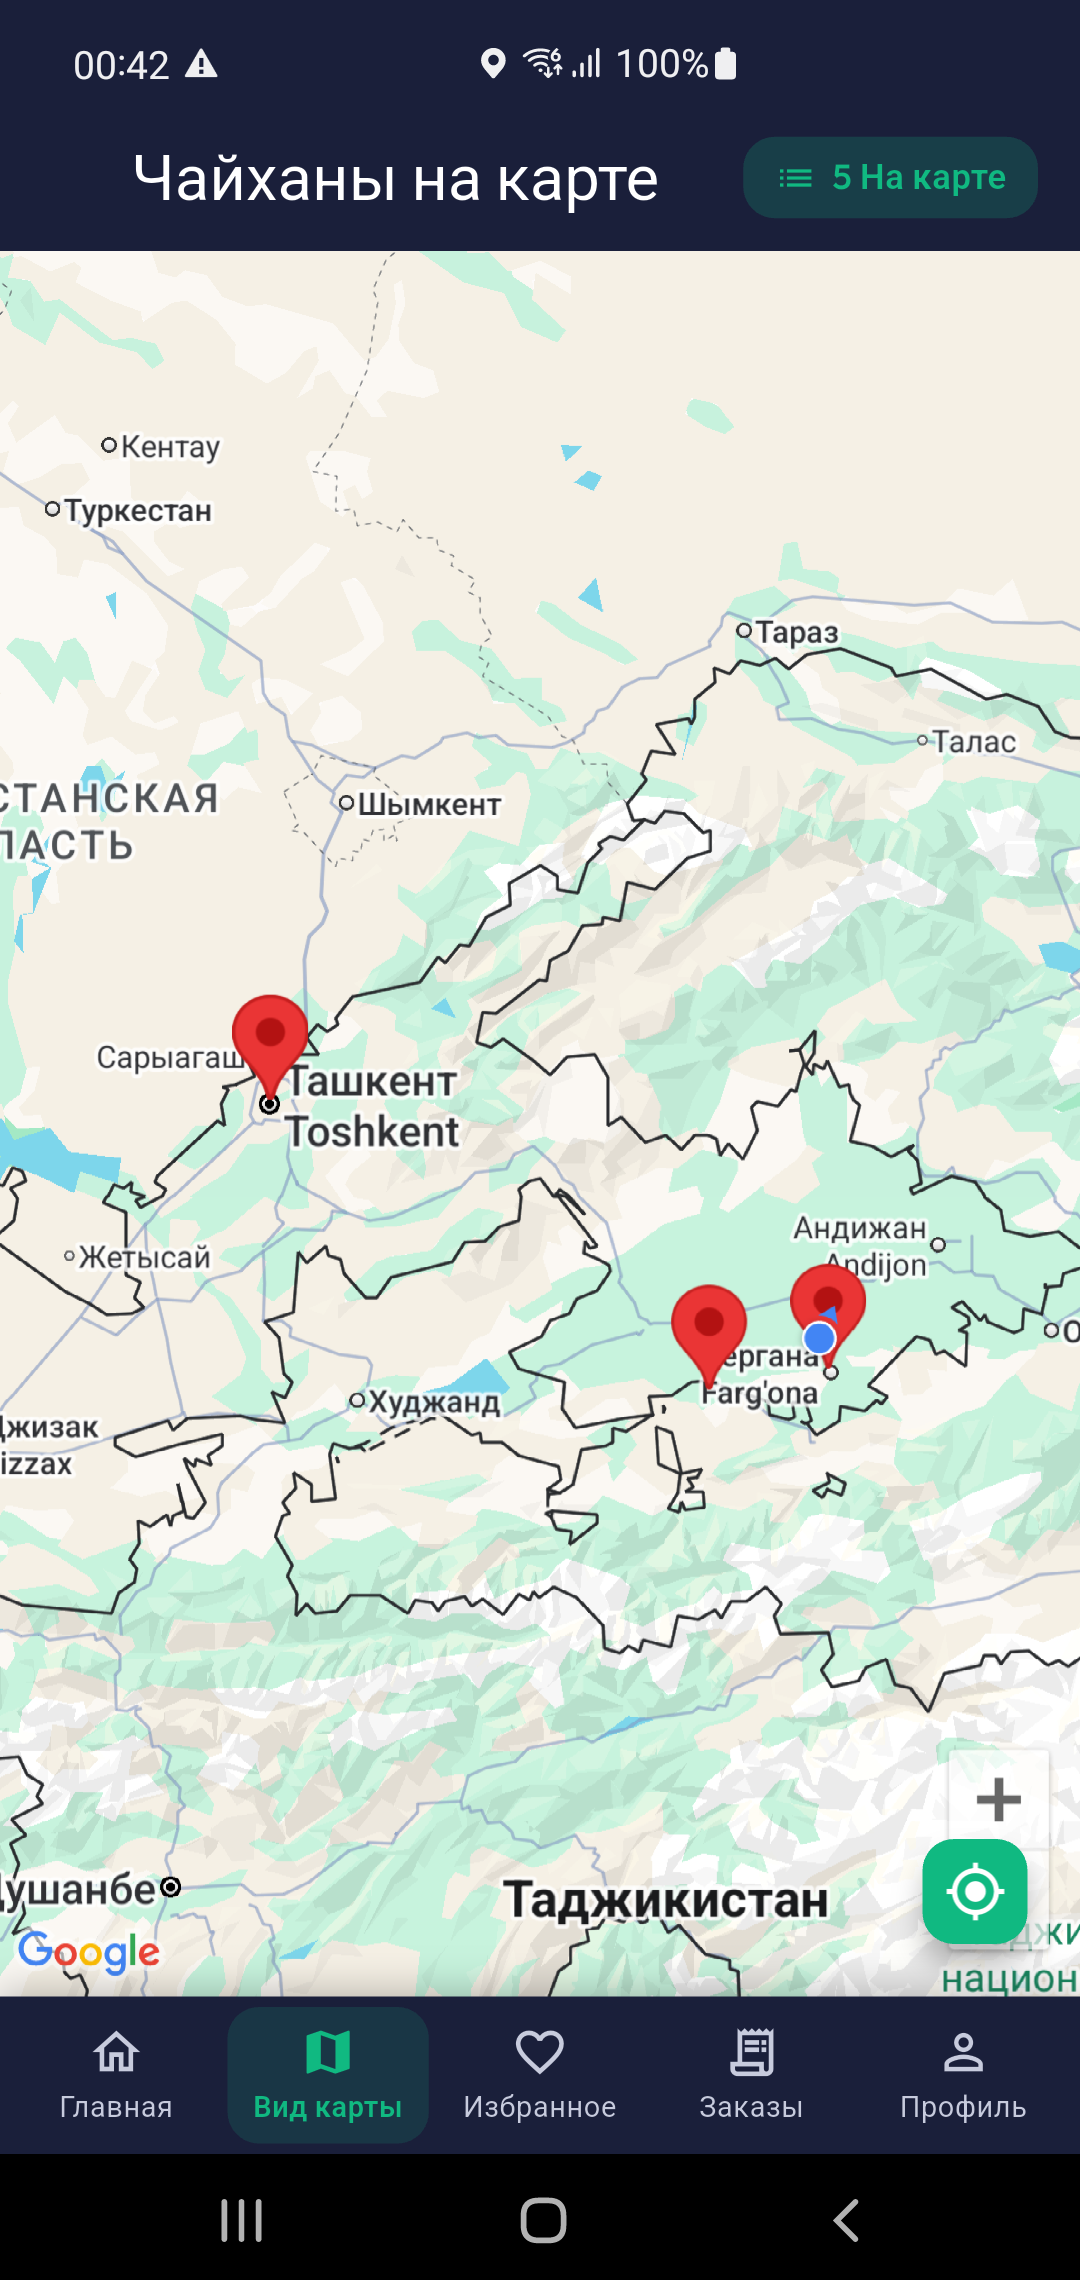
\includegraphics[width=0.4\textwidth]{b_chapters/chapter2/assets/screenshot_system.png}
  \figsource{CHOYXONA.UZ application screenshot.}
  \caption{Full-screen map view with bottom navigation bar showing the Map View tab active.}
  \label{fig:map-fullscreen}
\end{figure}

\cref{fig:map-fullscreen} demonstrates the full-screen map view with the bottom navigation bar.
Users can switch between list and map views while maintaining their current filters.
The map automatically positions to show all matching establishments, adjusting zoom level to fit results.


% =====================================================================
\section{Chapter Summary}
\label{sec:ch2-summary}

This chapter presented the technical foundation of the CHOYXONA.UZ application through five key areas:

First, \cref{sec:system-arch} described the three-layer architecture (presentation, business logic, data) that separates concerns and leverages Firebase's managed infrastructure to eliminate custom server maintenance.
The feature-based code organization ensures maintainability as the codebase grows.

Second, \cref{sec:database} detailed the Firestore data model with its primary collections (\texttt{users}, \texttt{choyxonas}, \texttt{bookings}, \texttt{reviews}), strategic denormalization for read optimization, composite indexing for multi-field queries, and role-based security rules enforcing authorization at the database level (\cref{tab:security-rules}).

Third, \cref{sec:ui-design} covered the Material Design~3 visual system with dual-theme support, bottom navigation architecture for five primary destinations, responsive layout breakpoints from compact phones to expanded tablets (\cref{tab:breakpoints}), and trilingual localization supporting Uzbek, Russian, and English.

Fourth, \cref{sec:realtime} explained the real-time synchronization mechanism using Firestore listeners and Flutter's \texttt{StreamBuilder}, the centralized \texttt{DataSyncProvider} for efficient stream sharing, offline persistence for unreliable connectivity, and transactional booking creation with optimistic updates.

Fifth, \cref{sec:maps} described Google Maps integration for geographic discovery, the Haversine formula for distance calculation (\cref{eq:haversine}), region-based filtering for planning scenarios, and external navigation app integration for directions.

These architectural foundations support the functional capabilities described in Chapter~3.
